% twocolumn を使うと2段組になる

%\documentclass[a4j,twocolumn]{jsarticle}        % -> platex
%\documentclass[a4j,twocolumn]{ujarticle}       % -> uplatex
\documentclass[uplatex]{jsarticle}   % -> uplatex + jsarticle

\usepackage{resume} % 他パッケージ,専用コマンド,余白の設定が書かれている

%%%%%%%%%%%%%%%%%%%%%%%%%%%%%%%%%%%%%%%%%%%%%%%%%%%%%%%%%%%%%%%%%%%%%%%%
% ヘッダ: イベント名,日付,所属,タイトル,氏名
%%%%%%%%%%%%%%%%%%%%%%%%%%%%%%%%%%%%%%%%%%%%%%%%%%%%%%%%%%%%%%%%%%%%%%%%

\pagestyle{plain}
\newcommand{\comment}[1]{}
\begin{document}
\twocolumn[
\beginheader{令和n年度 コンピュータサイエンス学部 ○○発表}{2022}{12}{15}{井上 研究室}
\title{モーションベースによるによる歩行感覚の提示によるユーザーへの影響}
\author{C0B20046 川東 隆継 (Kawahigashi Takatsugu) }
\endheader
]

\vspace{3mm}

 % 本番用ページ番号オフセット
\setcounter{page}{x}

%---------------------------------------------------------------------------
% 本文
%---------------------------------------------------------------------------


\section{はじめに}
現実世界においておこうは人間の活動に欠かせない移動手段の一つであり、VRでもコンテンツ
の種類を問わず、多く登場する。従来ではロコモーションインターフェイスのフットパッド型や、
トレッドミル型などの大掛かりな装置を用いることが多かったが近年では身体的負荷の低さや
姿勢の汎用性にメリットがある座位姿勢で利用するものも提案されているが立位姿勢と比較して
歩行感覚が生まれにくいという指摘もある。そこで本研究では、座位姿勢での仮想歩行体験について、
そのユーザ体験を総合的に評価した。特に、VRコンテンツへの適用を目的とし、歩行振動、
足ふみ操作、及び仮想の歩行者の存在がユーザー体験に与える影響を検証した。

\section{提案方法}
\subsection{実験装置・環境}
本実験ではエアコンプレッサ式のモーションベースを使用し、VR視聴用のHMDにはアイトラッキング
機能を有するVive Pro Eyeを用いた。
本実験はモーションベースが稼働するのに十分なスペースを確保できる環境で行い、
実験者はモーションベースの可動域外にて実験刺激を操作した。

\section{実験}
\subsection{概要}
実験条件は以下の\tabref{tab:zikken}に示すように歩行時振動、足踏み操作、
仮想の歩行者の有無が異なる条件C1から条件C4までの4条件であった。
なお、順序効果の影響を排除するため、体験する条件の順番は参加者によりランダマイズされた。

評価方法はアンケート、眼球運動、インタビューによって行った。
\begin{table}
  \centering
  % \scriptsize
  \caption{実験条件}
  \label{tab:fonts}
  \begin{tabular}[t]{|l|l|l|l|l|}
    \hline
     & 条件 & 条件 & 条件 & 条件\\
     & C1 & C2 & C3 &C4\\
    \hline
    歩行時振動 &なし&あり&あり&あり\\
    \hline
    足ふみ操作&なし&なし&あり&あり\\ 
    \hline
    仮想の歩行者&いない&いない&いない &いる\\
    \hline
  \end{tabular}
\end{table}
\subsection{歩行時振動の有無}
再現された歩行時の振動を付加した。以下の \figref{fig:my_label_2}、\figref{fig:my_label_3}にモーションベースに入力された角度 の推移 を示す。


\begin{figure}[b]
    \centering
    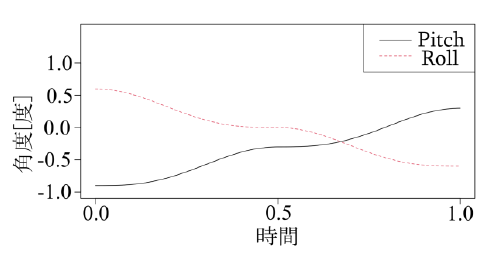
\includegraphics{rinkou_figure_2.png}
    \caption{実験環境}
    \label{fig:my_label_2}
\end{figure}

\begin{figure}[b]
    \centering
    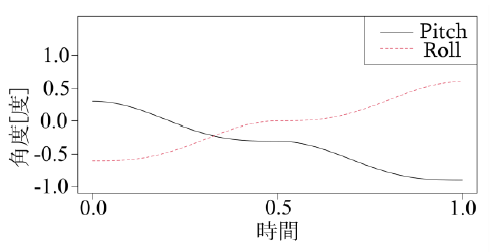
\includegraphics{rinkou_gigure_3.png}
    \caption{実験環境}
    \label{fig:my_label_3}
\end{figure}


\subsection{足踏み操作の有無}
足踏み操作がある条件では、参加者が左右のフットスイッチを交互に踏むことで仮想空間内を前進し、両方を踏むことで停止した。歩行時振動や 足 音の間隔は参加者の足踏みに同期させた。

足踏み操作がない条件では、自動的に仮想空間内
を前進した。参加者は両方のフットスイッチを踏んだまま
で刺激を体験した。

\subsection{仮想の歩行者の有無}
仮想の歩行者がいる条件では、仮想空間内に仮想
の歩行者を 7体配置した。うち 5体は参加者の前方か
ら参加者とすれ違い、 2体は後方から参加者を追い抜
くようにした。

\subsection{実験手順}
\figref{fig:my_label_4}に実験手順を示す。実験前にはキャリブレーシ
ョンとして、Vive Pro Eyeのアイトラッキング機能のキャリ
ブレーションと、参加者の平均的な足踏み時間の測定
を実施したのち、足踏み操作の練習を十分に行った。
本試行 は 4回行われた。各試行後には HMDを装着し
たままアンケートとインタビューへの回答を行 ったうえで、参加者が VR酔いの症状や疲労感を自覚していれば適宜休憩を挟み 、次の試行へと移った。

\begin{figure}[h]
    \centering
    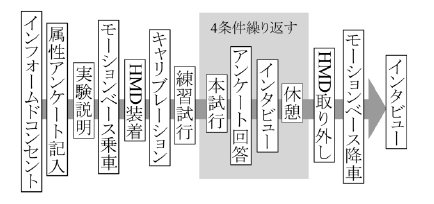
\includegraphics{rinkou_figure_4.png}
    \caption{実験環境}
    \label{fig:my_label_4}
\end{figure}
\section{実験結果}
\subsection{アンケート}
VR酔いに関する質問では、条件C2のスコアが他の条件と比較して有意に高かった。SAM\cite{文献18}情動価の結果では、条件C2のスコアが、条件C3、C4と比較して有意に低かった。SAM覚醒度の結果では、 歩行時振動のある条件で 有意に高かった。
歩行感覚に関する質問では すべての質問について、足踏み操作のある条件で有意に高かった。
仮想空間の認識に関する質問のうち、距離感覚と自身のスケール感では、条件間の有意差は確認できなかった。
速度感覚に関する質問では、条件C2のスコアが条件C3のスコアと比
較して有意に高い傾向があった 。条件C1、C4では実際歩行に近い速度知覚が得られていた。


\subsection{眼球運動}
眼球運動では条件C1より条件 C2、C4で有意に大きく、条件 C2より 条件 C4で有意に大きかった。全体を概して、刺激の要素が増えるほど瞳孔が拡大する傾向にあった。

視線移動量の指標である試行中の視線Yaw角の標準偏差の測定結果は名を外れ値として除外した。条
件C1と比較して条件C2、C3で有意に小さかった。

\section{おわりに}
本研究から、座位姿勢での仮想空間における歩行体
験について、歩行時振動、足踏み操作、仮想空間内に配置された仮想の歩行
者がユーザ体験に多様な変化、影響を与えることが明
らかになった。したがって、コンテンツ制作にあたっては
その制作意図に合わせて、装置や 映像の構成要素を
取捨選択することが 重要であると考えられた。







%---------------------------------------------------------------------------
% 本文終わり
%---------------------------------------------------------------------------

 % 参考文献
\bibliographystyle{junsrt}
\bibliography{ref}


\end{document}


%-----------------------------------------------------
% テンプレート
%------------------------------------------------------------------------------

%-----------
%% 箇条書き
%-----------
%\begin{itemize}
% \item
%\end{itemize}

%-------------------
%% 番号付き箇条書き
%-------------------
%\begin{enumerate}
% \item
%\end{enumerate}

%-----------
%% 図の表示
%-----------
%\begin{figure}[H]
% \centering
% \includegraphics[clip,width=7cm]{hoge.eps}
% \caption{図タイトル}\label{fig:hoge}
%\end{figure}

%-----------
%% 図の参照
%-----------
%\figref{fig:hoge}

%-----------
%% 表の作成
%-----------
%\begin{table}[H]
% \centering
% \caption{表タイトル}\label{tab:fuga}
% \begin{tabular}{|c|c|c|}\hline
%  hemo & piyo & fuga \\ \hline
%  hemo & piyo & fuga \\ \hline
% \end{tabular}
%\end{table}

%-----------
%% 表の参照
%-----------
%\tabref{tab:fuga}

%-----------
%% 参考文献
%-----------
%\begin{thebibliography}{9}
% \bibitem{piyo} 参考文献
%\end{thebibliography}

%-----------------
%% 参考文献の参照
%-----------------
%\cite{piyo}
